\section{The history database}

\begin{wrapfigure}{r}{0.4\textwidth}
  \vspace{-20pt}
  \begin{center}
    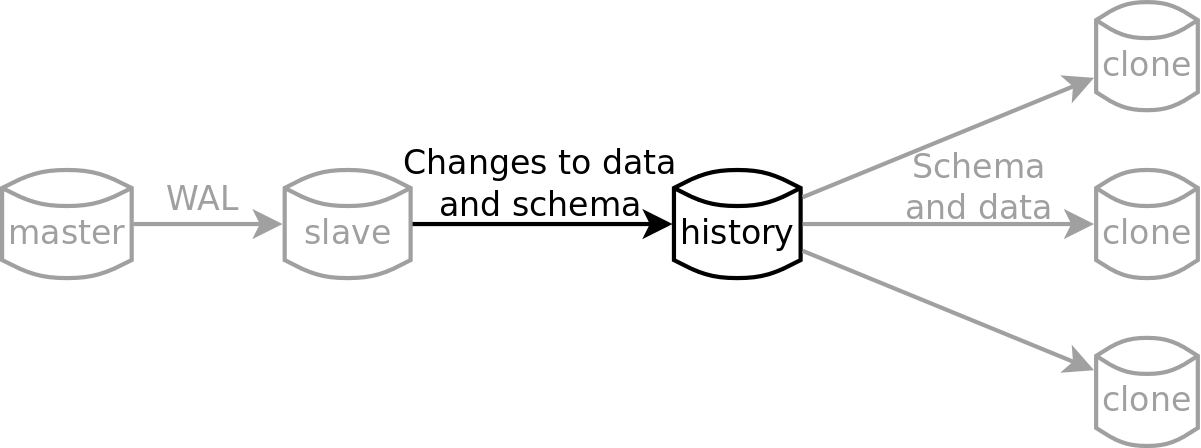
\includegraphics[width=0.38\textwidth]{img/architecture-history}
  \end{center}
  \vspace{-20pt}
  \caption{The history part of the architecture}
  \vspace{-10pt}
\end{wrapfigure}

The history database contains information about the schema of the master database and a copy of its data.
It contains multiple versions of the schema and data from the master, each transaction that alters the master database creates a history version.
It is used as a reference when the user creates a new clone database; the schema of the clone is created according to the information in the history database and its data is copied from the history.

The history database is created when the slave instance has been configured correctly.
It is a standard Postgres database that must have the same minor version as the master database.
That means that if the master runs on Postgres version 9.3.3 the history version must start with 9.3, see the Postgres documentation for further reference. % TODO add reference?

To initialize the history database the administrator runs the script \textit{history.py}.
This script starts by creating four tables, three of which are used to store information about the schema of the master database:

\begin{description}
  \item[marty\_updates]
    Contains meta information about each versions of the data in the history database.
  \item[marty\_schemas]
    Contains the name and ID of all schemas in the slave database.
  \item[marty\_tables]
    Contains the name and ID of the tables in the slave database and a reference to the schema they are in.
    It also stores the \textit{internal name} which is used for the data table in the history and the clone databases.
  \item[marty\_columns]
    Contains the name, number, type and length of each column in the tables.
    It also stores an internal name for the column that is used in the data tables in the history and clone databases.
\end{description}

The first table contains information about the history versions.
The other tables are used to store information about the database schema of the master database.
See tables \ref{table:marty-schemas} to \ref{table:marty-updates} for further information about each table in the history database.

\begin{table}[h]
  \centering
  \textbf{marty\_schemas}
  \begin{tabularx}{\textwidth}{llX}
    \textit{Column} & \textit{Type} & \textit{Description} \\
    \midrule
    \_ctid & tid & A reference to the pg\_namespace table in the slave database \\
    oid & oid & The ID of the schema in the slave database \\
    name & name & The name of the schema \\
    start & integer & First version where this schema is present in the database \\
    stop & integer & First version where this schema stops being present in the database \\
  \end{tabularx}
  \caption{The columns of the marty\_schemas table}
  \label{table:marty-schemas}
\end{table}

\begin{table}[h]
  \centering
  \textbf{marty\_tables}
  \begin{tabularx}{\textwidth}{llX}
    \textit{Column} & \textit{Type} & \textit{Description} \\
    \midrule
    \_ctid & tid & A reference to the pg\_class table in the slave database \\
    oid & oid & The ID of the table in the slave database \\
    name & name & The name of the table \\
    schema\_oid & oid & A reference to the schema that this table belongs to \\
    internal\_name & name & The name of the data tables in the history and clone databases \\
    start & integer & First version where this table is present in the database \\
    stop & integer & First version where this table stops being present in the database \\
  \end{tabularx}
  \caption{The columns of the marty\_tables table}
  \label{table:marty-tables}
\end{table}

\begin{table}[h]
  \centering
  \textbf{marty\_columns}
  \begin{tabularx}{\textwidth}{llX}
    \textit{Column} & \textit{Type} & \textit{Description} \\
    \midrule
    \_ctid & tid & A reference to the pg\_attribute table in the slave database \\
    table\_oid & oid & A reference to the table this column is in \\
    name & name & The name of the column \\
    number & int2 & The index of this column in the table (is it the first, second, third etc.) \\
    type & name & The type of the column (int, text, boolean etc.) \\
    internal\_name & name & The name of this column in the data tables in the history and clone databases \\
    start & integer & First version where this column is part of the table \\
    stop & integer & First version where this column stops being part of the table \\
  \end{tabularx}
  \caption{The columns of the marty\_tables table}
  \label{table:marty-columns}
\end{table}

\begin{table}[h]
  \centering
  \textbf{marty\_updates}
  \begin{tabularx}{\textwidth}{llX}
    \textit{Column} & \textit{Type} & \textit{Description} \\
    \midrule
    id & serial & Primary key - a unique ID for a version of the data \\
    time & timestamp & The date and time when this version was created in the history database \\
    mastertime & timestamp & The date and time of the transaction that created this version on the master database \\
  \end{tabularx}
  \caption{ The columns of the marty\_updates table}
  \label{table:marty-updates}
\end{table}
